\documentclass[tikz,border=10pt]{standalone}
\usepackage{tikz}
\usepackage{makecell}

\usetikzlibrary{arrows}
\usetikzlibrary{circuits.logic.US}
\usetikzlibrary{matrix}
\usetikzlibrary{positioning}
\usetikzlibrary{backgrounds}
\usetikzlibrary{decorations.pathreplacing, positioning, shapes.geometric, shapes.misc, shadows, fit}
\usetikzlibrary{shapes.geometric, shapes.symbols, arrows, shadows, fit, backgrounds, 3d, plotmarks, calc, intersections, matrix, patterns}

\tikzstyle{thin_arrow} = [draw,->,>=stealth]
\tikzstyle{arrow} = [thick,thin_arrow]
\begin{document} 

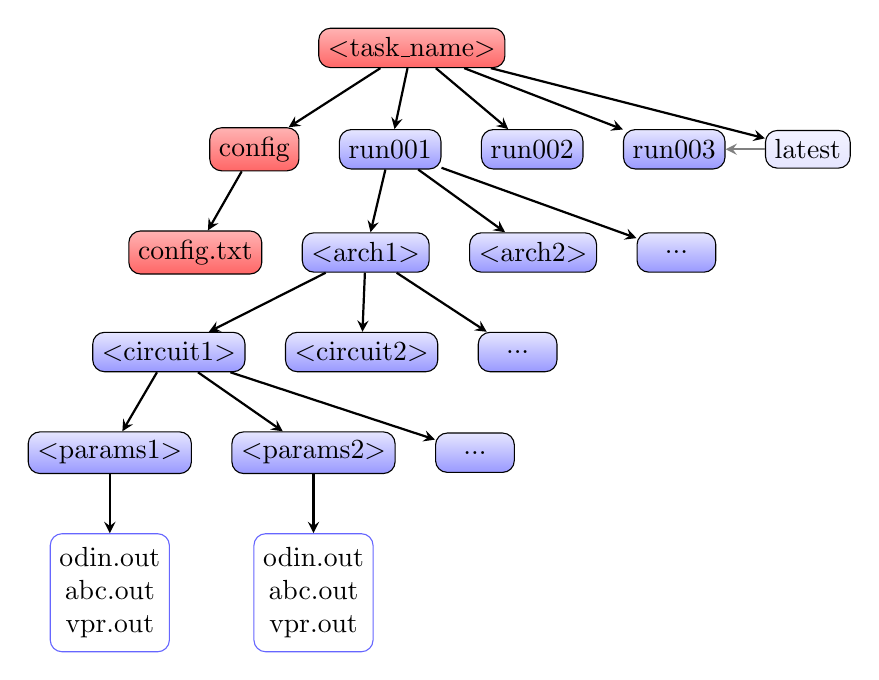
\begin{tikzpicture}[]
    \tikzstyle{task} = [draw, rectangle, rounded corners=1.5mm, top color=red!30, bottom color=red!60, minimum width=1cm, minimum height=0.5cm]
    \tikzstyle{run} = [draw, rectangle, rounded corners=1.5mm, top color=blue!10, bottom color=blue!40, minimum width=1cm, minimum height=0.5cm]
    \tikzstyle{run_result} = [draw=blue!60, rectangle, rounded corners=1.5mm]
    \tikzstyle{symlink} = [draw, rectangle, rounded corners=1.5mm, top color=blue!5, bottom color=blue!10,]

    \newcommand{\levelspace}{0.75cm}
    \newcommand{\nodespace}{0.5cm}
    \node[task](task) {\textless task\_name\textgreater };

    \node[task, below=\levelspace of task, xshift=-2cm](config) {config};
    \node[run, right=\nodespace of config](run001) {run001};
    \node[run, right=\nodespace of run001](run002) {run002};
    \node[run, right=\nodespace of run002](run003) {run003};
    \node[symlink, right=\nodespace of run003](latest) {latest};

    \node[task, below=\levelspace of config, xshift=-0.75cm](config_file) {config.txt};
    \node[run, right=\nodespace of config_file](arch1) {\textless arch1\textgreater };
    \node[run, right=\nodespace of arch1](arch2) {\textless arch2\textgreater };
    \node[run, right=\nodespace of arch2](archX) {...};

    \node[run, below=\levelspace of arch1, xshift=-2.5cm](cct1) {\textless circuit1\textgreater };
    \node[run, right=\nodespace of cct1](cct2) {\textless circuit2\textgreater };
    \node[run, right=\nodespace of cct2](cctX) {...};

    \node[run, below=\levelspace of cct1, xshift=-0.75cm](params1) {\textless params1\textgreater };
    \node[run, right=\nodespace of params1](params2) {\textless params2\textgreater };
    \node[run, right=\nodespace of params2](paramsX) {...};

    \node[run_result, below=\levelspace of params1] (result1) {\makecell{odin.out \\ abc.out \\ vpr.out}};
    \node[run_result, below=\levelspace of params2] (result2) {\makecell{odin.out \\ abc.out \\ vpr.out}};

    \draw[arrow] (task) -- (config);
    \draw[arrow] (task) -- (run001);
    \draw[arrow] (task) -- (run002);
    \draw[arrow] (task) -- (run003);
    \draw[arrow] (task) -- (latest);

    \draw[arrow, gray] (latest) -- (run003);

    \draw[arrow] (config) -- (config_file);
    \draw[arrow] (run001) -- (arch1);
    \draw[arrow] (run001) -- (arch2);
    \draw[arrow] (run001) -- (archX);

    \draw[arrow] (arch1) -- (cct1);
    \draw[arrow] (arch1) -- (cct2);
    \draw[arrow] (arch1) -- (cctX);

    \draw[arrow] (cct1) -- (params1);
    \draw[arrow] (cct1) -- (params2);
    \draw[arrow] (cct1) -- (paramsX);

    \draw[arrow] (params1) -- (result1);
    \draw[arrow] (params2) -- (result2);

\end{tikzpicture}
\end{document}
